%%%%%%%%%%%%%%%%%%%%%%%%%%%%%%%%%%%%%%%%%%%%%%%%%%%%%%%%%%%%
%%% LIVECOMS ARTICLE TEMPLATE
%%% ADAPTED FROM ELIFE ARTICLE TEMPLATE (8/10/2017)
%%%%%%%%%%%%%%%%%%%%%%%%%%%%%%%%%%%%%%%%%%%%%%%%%%%%%%%%%%%%
%%% PREAMBLE 
\documentclass[9pt]{livecoms}
% Use the 'onehalfspacing' option for 1.5 line spacing
% Use the 'doublespacing' option for 2.0 line spacing
% use the 'lineno' option for adding line numbers. 
% Please note that these options may affect formatting.

\usepackage{lipsum} % Required to insert dummy text
\usepackage[version=4]{mhchem} 
\usepackage{siunitx}
\DeclareSIUnit\Molar{M}
\newcommand{\versionnumber}{1.3}  % you should update the minor version number in preprints and major version number of submissions.
%%%%%%%%%%%%%%%%%%%%%%%%%%%%%%%%%%%%%%%%%%%%%%%%%%%%%%%%%%%%
%%% ARTICLE SETUP
%%%%%%%%%%%%%%%%%%%%%%%%%%%%%%%%%%%%%%%%%%%%%%%%%%%%%%%%%%%%
\title{Best Practices for Transport Properties : v\versionnumber}

%Edward Maginn (ejmaginn), Richard Elliott, Sunny Hwang, Daniel Roe (GitHub: drroe), Rich Messerly (ramess101)

\author[1*,\authfn{1}\authfn{3}]{Edward Midname Maginn}
\author[2\authfn{1}\authfn{4}]{Daniel Midname Roe}
\author[3\authfn{1}\authfn{5}]{J. Richard Elliott}
\author[4\authfn{1}\authfn{6}]{Richard Alma Messerly}
\author[5\authfn{1}\authfn{7}]{Daniel Midname Carlson}
\affil[1]{The University of Notre Dame}
\affil[2]{Roe's institution}
\affil[3]{The University of Akron}
\affil[4]{National Institute of Standards and Technology}
\affil[5]{Brigham Young University}

\corr{Maginn's email}{EM}  % Correspondence emails.  Second {} are the appropriate authors initials. 
\corr{Roe's email}{DR}
\corr{Elliott's email}{JRE}
\corr{richard.messerly@nist.gov}{RAM}
\corr{Carlson's email}{DC}

\contrib[\authfn{1}]{These authors contributed equally to this work}
\contrib[\authfn{2}]{These authors also contributed to this work}

\presentadd[\authfn{3}]{Maginn's Department, Institute, Country}
\presentadd[\authfn{4}]{Roe's Department, Institute, Country}
\presentadd[\authfn{5}]{Elliott's Department, Institute, Country}
\presentadd[\authfn{6}]{Thermodynamics Research Center, National Institute of Standards and Technology, USA}
\presentadd[\authfn{7}]{Chemical Engineering Department, Brigham Young University, USA}

%%%%%%%%%%%%%%%%%%%%%%%%%%%%%%%%%%%%%%%%%%%%%%%%%%%%%%%%%%%%
%%% ARTICLE START
%%%%%%%%%%%%%%%%%%%%%%%%%%%%%%%%%%%%%%%%%%%%%%%%%%%%%%%%%%%%

\begin{document}

\maketitle

\begin{abstract}
%Please provide an abstract of no more than 250 words. Your abstract should explain the main contributions of your article, and should not contain any material that is not included in the main text.

The ability to predict transport properties (i.e. diffusivity, viscosity, conductivity) is one of the primary benefits of molecular simulation. Although most studies focus on the accuracy of the simulation output compared to experimental data, such a comparison primarily tests the adequacy of the force field (i.e. the model). By contrast, the reliability of different simulation methodologies for predicting transport properties is the focus of this manuscript. Unfortunately, obtaining reproducible estimates of transport properties from molecular simulation is not as straightforward as static properties. Therefore, this manuscript discusses the best practices that should be followed to ensure that the simulation output is reliable, i.e. is a valid representation of the force field implemented.

There are two classes by which transport properties are predicted: equilibrium molecular dynamics (EMD) and non-equilibrium molecular dynamics (NEMD). This manuscript presents the best practices for EMD, leaving NEMD for a future publication. As self-diffusivity and shear viscosity are the most prevalent transport properties found in the literature, the discussion will also be limited to these properties with the expectation that future publications will discuss best practices for thermal conductivity, ionic conductivity, and transport diffusivity.

\end{abstract}

%List of people to contact: Peter Cummings, Richard Rowley, Joachim Gross, Raj Khare, Richard Sadus, Ioannis Economou, Jadran Vrabec, Daniel Carlson, Chris Iocavella (any other Richards we can come up with)


\section{Outline: Not included in publication}

% This outline is currently not implemented.
General outline of equilibrium methods of self-diffusivity and viscosity for liquids:
\begin{enumerate}
	\item Introduction
	\item Discussion of different methods within EMD (Green-Kubo, Einstein)
	\item Summary of checklist for each property and method 
	\item General checklist items
	\item Diffusion
	\begin{enumerate}
		\item Diffusion specific checklist items
		\item Brief discussion of why we recommend Einstein over Green-Kubo?
		\begin{enumerate}
			\item Simulation setup that is specific to Einstein/diffusion 
		    \item Data analysis specific to Einstein/diffusion
		    \item Common pitfalls for Einstein/diffusion
		\end{enumerate}
		\begin{enumerate}
			\item Simulation setup that is specific to Green-Kubo/diffusion 
			\item Data analysis specific to Green-Kubo/diffusion
			\item Common pitfalls for Green-Kubo/diffusion
		\end{enumerate}	
	\end{enumerate}
	\item Viscosity
	\begin{enumerate}
		\item Viscosity specific checklist items
		\item Brief discussion of why we recommend Green-Kubo over Einstein?
		\begin{enumerate}
			\item Simulation setup that is specific to Green-Kubo/viscosity
			\item Data analysis specific to Green-Kubo/viscosity
			\item Common pitfalls for Green-Kubo/viscosity 
		\end{enumerate}
        \begin{enumerate}
        	\item Simulation setup that is specific to Einstein/viscosity
        	\item Data analysis specific to Einstein/viscosity
        	\item Common pitfalls for Einstein/viscosity 
        \end{enumerate}
	\end{enumerate}
\end{enumerate}


\section{Introduction}

Transport properties describe the rates at which mass, momentum, heat or charge move through a given substance. They involve mean squared displacements (MSDs) of molecules as the system evolves dynamically. In general, these properties can be computed by equilibrium molecular dynamics (EMD) or by non-equilibrium molecular dynamics (NEMD) methods. The EMD methods involve post-processing of a standard molecular dynamics (MD) trajectory while NEMD methods require modifications of the underlying equations of motion and/or boundary conditions of the system. Many codes such as LAMMPS (\cite{LAMMPS}) and GROMACS (\cite{GROMACS}) have analysis tools that automatically estimate transport properties from an EMD or NEMD simulation, but there are often insufficient checks as to whether the actual underlying simulations are adequate for making these estimates. As Berk Hess has said in a forum post on using the GROMACS ``energy -vis'' option for calculating viscosity, ``...it will give nonsense unless you know exactly what you are doing'' \cite{HessForum}. For this reason, following best practices is imperative to ensure that meaningful predictions are obtained. The purpose of this document is to improve the quality of published results and to reduce the time required for a novice in the field to obtain meaningful and reliable results.

In addition to the present manuscript, we highly recommend reviewing this list of existing resources:
\begin{enumerate}
	\item Text books:
	\begin{enumerate}
		\item \cite{Allen1987}, pages 58-64, 204-208, and 240-256
		\item \cite{Frenkel2002}, pages 87-90 and 509-523
		\item \cite{Leach2001}, pages 374-382
	\end{enumerate}
	\item Class notes
	\begin{enumerate}
		\item http://paros.princeton.edu/cbe422/md2.pdf
		\item http://paros.princeton.edu/cbe520/Transport.pdf
		\item https://engineering.ucsb.edu/~shell/che210d/Computing\_properties.pdf
		\item https://www3.nd.edu/~ed/notes.pdf
		\item http://www.eng.buffalo.edu/~kofke/ce530/Lectures/Lecture12.ppt.pdf
	\end{enumerate}
	\item Published articles
	\begin{enumerate}
		\item \cite{Hess2002}
		\item \cite{Chen2009}
		\item \cite{Ungerer2007}
		\item \cite{Nieto2015}, pages 13139-13140
	\end{enumerate}
	\item Software manuals
	\begin{enumerate}
		\item \cite{GROMACS}
		\item \cite{LAMMPS}
	\end{enumerate}
\end{enumerate}
Most text books and class notes provide a thorough discussion of EMD/NEMD theory with little discussion of practical considerations. Review articles tend to focus on the numerical advantages and disadvantages of different methods but assume that the reader already understands the subtleties of implementing each method. Furthermore, although software manuals describe some of the theory and implementation of these methods in their respective environments, the documentation is typically insufficient for someone not familiar with best practices for estimating transport properties. This document supplements the existing literature by providing a succinct checklist and common pitfalls.

\section{Equilibrium Molecular Dynamics (EMD) for Estimating Transport Properties}

It is most convenient to consider compiling the transport properties as an implicit part of any equilibrium MD simulation. The added computational overhead is relatively small, especially for the self-diffusivity. The main caveat is that longer simulations than normal may be required to achieve reasonable averages. 

The general formula for computing a transport property via an EMD simulation is given as

\begin{equation} \label{eq:Green-Kubo}
\gamma = \int_{0}^{\infty}dt\langle\dot{\xi}(t)\dot{\xi}(0)\rangle
\end{equation}
where $\gamma$ is the transport coefficient (within a multiplicative constant) and $\xi$ is the perturbation in the Hamiltonian associated with the particular transport property under consideration and $\dot{\xi}$ signifies a time derivative. Integrals of the form given by Equation \ref{eq:Green-Kubo} are known as “Green-Kubo” integrals. It is easy to show that an integrated form of Equation \ref{eq:Green-Kubo} results in an equivalent expression for $\gamma$ known as the “Einstein” formula

\begin{equation} \label{eq:Einstein}
\gamma = \lim_{t\to\infty} \frac{\langle (\xi(t)-\xi(0))^2 \rangle}{2t} = \frac{1}{2} \lim_{t\to\infty} \frac{d}{dt} \langle (\xi(t)-\xi(0))^2 \rangle
\end{equation}
where the derivative form is often preferred.

For self-diffusivity, $\xi$ is the Cartesian atom position and the time correlation function, $\dot{\xi}$, in Equation \ref{eq:Green-Kubo} is of the molecular velocities. For the shear viscosity, the integral in Equation \ref{eq:Green-Kubo} is of the time correlation of the off-diagonal elements of the stress tensor. For the thermal conductivity the integral is over the energy current, and for the electrical conductivity the integral is over the electric current. The relevant equations for self-diffusivity and shear viscosity are provided in Table \ref{tab:EMD_equations}.

% I think this table could be useful -ramess101

%\begin{table}[bt]
%	\caption{\label{tab:EMD_equations}Equilibrium molecular dynamics equations.}
%	% Use ``S'' column identifier to align on decimal point 
%	% ``l'' left aligns text in the column
%	% ``r'' right aligns text in the column
%	% ``c'' right aligns text in the column
%	% & separates columns, \\ ends the row.
%	
%	\begin{tabular}{l l l l l} 
%		\toprule
%		Property & $\gamma$          & $\xi$                        & Equation \ref{eq:Green-Kubo}    & Equation \ref{eq:Einstein}     \\
%		\midrule
%		Self-diffusion     & $D$ & $x$          & $\int_{0}^{\infty}dt\langle v_{x,i}(t) v_{x,i}(0)\rangle$    & $\frac{1}{2t}\langle (x_i(t)-x_i(0))^2 \rangle$   \\
%		Shear viscosity     & $\eta$       & $x v_y$           & $\beta V \int_{0}^{\infty}dt\langle P_{x,y}(t) P_{x,y}(0)\rangle$    & $\frac{m^2\beta}{2t}\langle (x_i(t)v_{y,i}(t)-x_i(0)v_{y,i}(0))^2 \rangle$  \\
%		Thermal conductivity      & $\lambda$      & $x E$              & $ \frac{k\beta^2}{V} \int_{0}^{\infty}dt\langle S_{x}(t) S_{x}(0)\rangle$    & $\frac{k\beta^2}{2Vt}\langle \left(x_i(t)(E_i(t)-\langle E \rangle)-x_i(0)(E_i(0)-\langle E \rangle)\right)^2 \rangle$  \\
%		\bottomrule
%	\end{tabular}
%$P_{x,y}(t) = \frac{1}{V} \sum_{i=1}^{N} \left( \frac{p_{x,i}(t)p_{y,i}(t)}{m} + x_i(t) f_{y,i}(t) \right)$
%\newline
%$S_{x}(t) = \frac{d}{dt} \sum_{i=1}^{N} \left( x_i(t) (E_i(t) - \langle E \rangle) \right)$.
%\end{table}

% Since this paper focuses on diffusion and viscosity I have removed conductivity. I also modified the equations somewhat. -RAM
%\begin{table}[bt]
%	\caption{\label{tab:EMD_equations}Equilibrium molecular dynamics equations.}
%	% Use ``S'' column identifier to align on decimal point 
%	% ``l'' left aligns text in the column
%	% ``r'' right aligns text in the column
%	% ``c'' right aligns text in the column
%	% & separates columns, \\ ends the row.
%	
%	\begin{tabular}{l l l l l} 
%		\toprule
%		Property & $\gamma$          & $\xi$                        & Equation \ref{eq:Green-Kubo}    & Equation \ref{eq:Einstein}     \\
%		\midrule
%		Self-diffusion     & $D$ & $\alpha$          & $\int_{0}^{\infty}dt\langle v_{\alpha,i}(t) v_{\alpha,i}(0)\rangle$    & $\frac{1}{2t}\langle (\alpha_i(t)-\alpha_i(0))^2 \rangle$   \\
%		Shear viscosity     & $\eta$       & $\alpha \dot{\beta}$           & $\frac{V}{k_bT} \int_{0}^{\infty}dt\langle P_{\alpha,\beta}(t) P_{\alpha,\beta}(0)\rangle$    & $\frac{m^2}{2k_bTVt}\langle (\alpha_i(t)\dot{\beta_i}(t)-\alpha_i(0)\dot{\beta_i}(0))^2 \rangle$  \\
%		\bottomrule
%	\end{tabular}
%\newline
%$P_{\alpha,\beta}(t) = \frac{1}{V} \sum_{i=1}^{N} \left( \frac{p_{\alpha,i}(t)p_{\beta,i}(t)}{m} + \alpha_i(t) \ddot{\beta_i}(t) \right)$
%\newline
%$\alpha$, $\beta = x, y, $ or $z$ coordinates
%\end{table}

\begin{table}[bt]
	\caption{\label{tab:EMD_equations}Equilibrium molecular dynamics equations.}
	% Use ``S'' column identifier to align on decimal point 
	% ``l'' left aligns text in the column
	% ``r'' right aligns text in the column
	% ``c'' right aligns text in the column
	% & separates columns, \\ ends the row.
	
	\begin{tabular}{l l l l l} 
		\toprule
		Property & $\gamma$          & $\xi$                        & Green-Kubo (Equation \ref{eq:Green-Kubo})    & Einstein (Equation \ref{eq:Einstein})     \\
		\midrule
		Self-diffusivity     & $D$ & $r$          & $\frac{1}{3} \int_{0}^{\infty}dt\langle \frac{1}{N} \sum_{i=1}^{N} v_{\alpha,i}(t) v_{\alpha,i}(0)\rangle$    & $ \displaystyle \frac{1}{6} \lim_{t\to\infty} \frac{d}{dt} \langle \frac{1}{N} \sum_{i=1}^{N} |r_i(t)-r_i(0)|^2 \rangle$   \\
		Shear viscosity     & $\eta$       & $r_\alpha v_\beta$           & $\frac{V}{k_bT} \int_{0}^{\infty}dt\langle P_{\alpha,\beta}(t) P_{\alpha,\beta}(0)\rangle$    & $ \displaystyle \frac{V}{2k_bT} \lim_{t\to\infty} \frac{d}{dt} \langle (P_{\alpha,\beta}(t)-P_{\alpha,\beta}(0))^2 \rangle$  \\
		\bottomrule
	\end{tabular}
	\newline
	%$P_{\alpha,\beta}(t) = \frac{1}{V} \sum_{i=1}^{N} \left( \frac{p_{\alpha,i}(t)p_{\beta,i}(t)}{m} + \alpha_i(t) \ddot{\beta_i}(t) \right)$
	$P_{\alpha,\beta}(t) = \frac{1}{V} \sum_{i=1}^{N} \left( m v_{\alpha,i}(t) v_{\beta,i}(t) + r_{\alpha,i}(t) f_{\beta,i}(t) \right) , \alpha \ne \beta$
	\newline
	$\alpha$, $\beta = x, y, $ or $z$ Cartesian coordinates
\end{table}

Transport properties are estimated by numerical integration of Equation \ref{eq:Green-Kubo} or calculating the slope of Equation \ref{eq:Einstein} with respect to time. Both methods involve some judgment on the part of the user and results can vary depending on where the slope is taken (Einstein approach) and for how long the integral is carried out (Green-Kubo approach). Some recent work has suggested some guidelines for how to compute an objective estimate of the viscosity using the Green-Kubo approach. Similar methods for estimating other transport properties from Equations \ref{eq:Green-Kubo} or \ref{eq:Einstein} should be possible to develop. As no single best practice can be recommended for the region over which the slope or integral is calculated, it is important to justify how this decision was made. Furthermore, it is critical to quantify the degree of variability in the estimated property that arises from varying the time interval included in the data analysis. 

In practice, several tricks-of-the-trade are employed to reduce fluctuations and, thereby, the standard deviation. For self-diffusivity, it is a standard practice to average the mean-square-displacement or velocity autocorrelation function over all $N$ molecules (see Table \ref{tab:EMD_equations}). For shear viscosity, it is not possible to average over the number of particles because viscosity is a collective property that depends on the pressure/stress tensor of the system. For self-diffusivity, it is also standard practice to average the x, y, and z displacements or velocities. For viscosity, the recommended practice is to use multiple components from the pressure/stress tensor. For example, although early studies only implemented a single off-diagonal component (typically xy), the common practice in recent studies is to use all three off-diagonal (xy, yz, zx) and sometimes three additional modified diagonal terms of the pressure/stress tensor. Finally, for both self-diffusivity and shear viscosity it is common to average over multiple time origins $(t_0)$. It is important that the difference between subsequent $t_0$ values $(\delta t_0)$ be longer than the correlation time so that the different time intervals are independent.

An important implicit assumption in Equations \ref{eq:Green-Kubo} and \ref{eq:Einstein} is that the time over which these expressions are evaluated is much larger than the correlation time of the variable $\xi$. This assumption is often satisfied easily for simple liquids, where relaxation times are fast, but becomes problematical for systems with sluggish dynamics. Obtaining reliable results with reasonable uncertainties can require simulations that are much longer than the longest relaxation times in the system, which are often unknown at the start of a simulation. Therefore, insufficient simulation time is a common pitfall in estimating transport properties. To avoid this pitfall, we recommend performing a series of progressively longer simulations to determine if the estimated values deviate significantly with increasing simulation time.

% Do we have a recommendation here for how to overcome this? Perhaps varying the simulation time to observe any change in the property value? -RAM  

Although both Equation \ref{eq:Green-Kubo} (Green-Kubo) and Equation \ref{eq:Einstein} (Einstein) are theoretically rigorous, in practice one method is often preferred depending on the property being estimated. In the case of self-diffusivity, we recommend the Einstein (MSD) approach. By contrast, for shear viscosity we typically recommend Green-Kubo, although for some systems the Einstein approach may be preferable. Precision and reproducibility of the estimated value are key factors for selecting between the Green-Kubo or Einstein methods. For this reason, we emphasize the importance of proper data analysis and uncertainty quantification.

\subsection{Checklist for Equilibrium Einstein Approach for Self-Diffusivity}

%I think that we should have this just as a general Einstein approach section and then if anything is specific to Self-Diffusivity we move it to a new section -ramess101

We recommend the Einstein approach for computing self-diffusivity as it is robust and the most commonly used method. However, we also recommend validating that the Green-Kubo method provides similar estimates. Although systematic deviations are often observed between the two methods, if the analysis is done properly the values should agree within their statistical uncertainties \cite{Kondratyuk2016,Liu2012,Mondello1997}. 

\begin{enumerate}
	\item Ensemble - for a liquid solution, it is safest to run in the microcanonical (NVE, constant number of molecules, volume, energy) ensemble. %Although this may be the best practice, it appears to me that a large number of practitioners run their production simulations in the NPT ensemble. Should we point this out? I.e. should we say something like "although it is common to see values reported from the NPT ensemble..."? That way the reader will know why our recommendation seems to differ from what they find in the literature. -ramess101
	% What about for the gas phase? -RAM
	\begin{enumerate}
		\item Generally you want a self-diffusivity at a specified temperature (T) and pressure (P). This requires performing a series of simulations in different ensembles:
		\begin{enumerate}
			\item NPT ensemble at desired T and P until equilibrium is well sampled (link to equilibration document)
			\item NVT ensemble where the volume is set such that the density is the average density computed from the NPT run
			\item NVE ensemble where the final configuration of the NVT run is used as the initial configuration
		\end{enumerate}
		The average pressure and temperature for the NVE production run are computed and should be close to (but not exactly the same) as the input P and T to the original NPT run. These average pressures and temperatures must be reported along with the self-diffusivity. The user should generate multiple starting states that can be used to determine error estimation (see item \ref{item:uncertainty}).
		% Do we really just want the last configuration? Should we randomly select a configuration from production? Or a few configurations to run in parallel? Or somehow find an "average" configuration? My concern is just, what if the last configuration happens to be a higher energy sample (or lower probability if coming at it from a Monte Carlo point of view)? -ramess101
		\item For systems that require anisotropic pressure control (e.g. membranes etc), use of a barostat/thermostat that maintains the correct isothermal/isobaric ensemble (e.g. extended system, Langevin piston) is required.
	\end{enumerate}
    \item Ensure energy conservation (via adjusting time step, constraint tolerances, etc) (Link to document about initializing NVE in the right “ballpark.”) 
    \item Output frequency should be sufficient to have around 1000 data points over the entire MSD. Typical recommendations are every NEED RECOMMENDATION
    \item Use ``unwrapped coordinates'' of molecule center of mass to determine mean squared displacement; can also track all atomic coordinates and ensure consistency with center of mass.
    %Does ``unwrapped coordinates'' require an explanation? Do most open-source simulation packages have the option to track ``unwrapped coordinates''? -ramess101
    \item Finite size effects tend to be significant and need to be accounted for, i.e. system size corrections must be applied. For example, see \cite{Yeh2004,Moultos2016}. Some correction approaches require that the viscosity be calculated first or that multiple simulations are run with varying box sizes / number of molecules in order to estimate the infinite size limit of the self-diffusivity.
    \item Multiple time origins used for MSD (block averaging) - is there a best practice?
	\item Compute the diffusion coefficient separately in each dimension, i.e. $D_{xx}$, $D_{yy}$, and $D_{zz}$. For a homogeneous system, $D_{xx}$, $D_{yy}$, and $D_{zz}$ should be equal and provides a useful validation of simulation quality. The variation in these values can be used for a rough estimate of the statistical uncertainty, although more rigorous methods for uncertainty estimation are recommended (see item \ref{item:uncertainty}).
	\item In order to obtain reliable estimates of D, it is important to consider how the linear regression is performed for the MSD with respect to time (Equation 2). Specifically, the time interval that is included in the regression can have a significant impact on the predicted value of D. We recommend that only the “middle” of the MSD be used in the fit. Short time must be excluded as it follows a ballistic trajectory, while very long time is excluded due to the increased noise. Currently, we are unaware of an objective approach for defining the “middle” region. Until such an approach exists, we recommend that the author reports how the region was selected and how much variability in D can be attributed to the choice of this region. In addition, the uncertainty in the fit of the slope should be reported.
	What about when the middle region is subdiffusive like in Figure \ref{fig:KondratyukFig2}?
	%How do you fit the MSD (what time interval do you use?) Short time is ballistic trajectory; very long time you get noise, so you need to fit to the “middle” of the MSD. We need to define protocols for how to objectively define this. You should compute the uncertainty in the fit of the slope. Report how the line was fit and associated variables. Is there literature on this? We need to come up with a recommendation for how to do this objectively and consistently. 
	% If there is no published literature on the subject, rather than provide a recommendation, should we just present the issue that they need to be aware of? -ramess101
	% I think we should have a figure to help visualize this -ramess101
	\item Simulation length needed depends on number of molecules for which transport properties are desired. Fewer molecules requires more simulation time and vice versa. Regardless, the simulation must be long enough so that the molecules are in the diffusive regime. One way of checking this is if the slope of a plot of ln(MSD) vs ln (t) = 1. Other heuristics are: is the MSD sufficiently large (larger than the square of the radius of gyration of the molecule at the low end, and larger than the square of half the box length at the high end).
	\item Compute statistical uncertainty by running independent replicates (using multiple starting states from NPT run at desired temperature) and taking the standard deviation (what do the uncertainty people say?) How many replicates do we recommend? Link to Sampling/Uncertainty doc. Use Zwanzig/Szabo four-time correlation for MSD averaging…. \label{item:uncertainty}
	\item Calculating diffusion in membrane systems with PBC require some additional consideration, use of Saffman-Delbruck model: see http://pubs.acs.org/doi/abs/10.1021/acs.jpcb.6b09111, also http://dx.doi.org/10.1063/1.4932980
	\item Handling potential truncation: shifted force, shifted potential, cutoff, long range corrections. We need to come up with recommendations on this.
\end{enumerate}

FYI: Richard Elliot I developed a database for self-diffusivity that covered all experimental data from the literature as far as he could find. It is included as supporting information in Ind. Eng. Chem. Res. 2010, 49, 3411–3423. This paper provides a generalized correlation of the quantity rho*D (g/cm-s) of n-alkanes at all molecular weights, temperatures, and densities below the entanglement threshold. This semi-empirical correlation is used as the basis for correlating non-alkanes as well. Accuracy diminished for associating compounds, but experimental data were relatively few in number for associating compounds.

\begin{figure}[htb!]
	\centering
	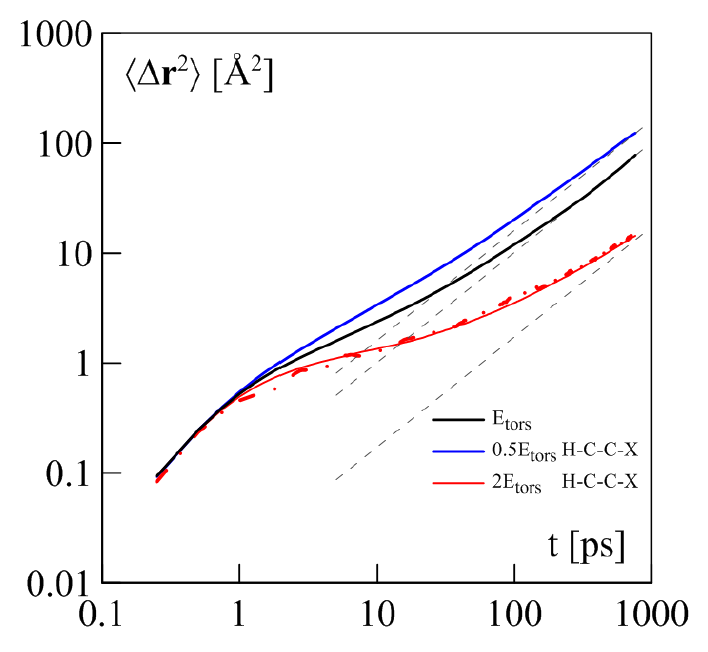
\includegraphics[width=3.2in]{figures/KondratyukFig2.png}
	\caption{}
	\label{fig:KondratyukFig2}
\end{figure}

\subsection{Equilibrium Green-Kubo Approach for Self-Diffusivity}

Many of the same best practices for the Einstein approach apply to the Green-Kubo method. Specifically, items 1, 2, 4, 5, 6, 7, and 12 from the previous Section are also applicable to the Green-Kubo approach. Some key differences are:

\begin{enumerate}
	\item Need to write velocities instead of positions, and the frequency should be much higher because the integral of the velocity autocorrelation function decays rapidly. Recommend writing every 5 fs. 
	\item Integrate the VACF numerically, providing details of how this is done.
	\item Plot the running integral vs time. The data are best at short time and noise takes over at long times. Like with the MSD, a cut-off needs to be determined when you decide the integral has converged. It is important to report how sensitive the estimate is to this cut-off time. \label{item:GreenKuboDiffusivity}
	\item Independent simulations should be run and each integral can be averaged together to obtain a smoothed integral. With these replicate simulations, we recommend that the uncertainty be determined using a bootstrap methodology:
	\begin{enumerate}
		\item Randomly selecting (with replacement) from the set of replicate simulations
		\item Calculating the average integral from this random set
		\item Estimating the self-diffusivity as described in item \ref{item:GreenKuboDiffusivity}
		\item Repeat steps a)-c) thousands of times
		\item Generate distribution of the estimated values of self-diffusivity 
		\item Compute uncertainty by integrating distribution at desired confidence level
	\end{enumerate}
\end{enumerate}

\subsection{Checklist for Equilibrium Green-Kubo Approach for Viscosity}

Similar to self-diffusivity, EMD for viscosity is straightforward but its reliability compared to experimental data has not been evaluated with a comprehensive database. Many more experimental data are available for viscosity than for self-diffusivity. Anecdotal studies with small databases show encouraging results, but deviations from experiment can range from 5-35\% even when results are said to be “good.” Nieto-Draghi et al. provide a useful review of the status quo \cite{Nieto2015}. EMD may deviate 2x more than NEMD from experimental data; hydrogen bonding throws in complications that may require empirical corrections. 

% I don't think we want to talk about comparison to experimental data. We are not really concerned about if diffusivity or viscosity are accurately predicted relative to experiment, we just want to present the best methods for obtaining reproducible/honest results. In addition, you can predict viscosity more accurately if you parameterize your force field for such a purpose. -ramess101

% I am unaware of this - can a citation be given? -ejmaginn

We recommend the Green-Kubo approach for predicting viscosity. This appears to be the most popular EMD method found in the literature. More importantly, less arbitrary data analysis methods exist that improve the reliability and reproducability. 

Although the popularity of NEMD methods for predicting viscosity has increased in recent years, \cite{Chen2009} demonstrate that EMD methods can be of equal accuracy and reliability to NEMD as long as best practices (i.e. thorough data analysis) are implemented. That being said, EMD works best for fluids with relatively low viscosity (less than 50 cP). Higher viscosity systems are extremely difficult to compute with EMD and so NEMD methods are often preferred in this case.

\begin{enumerate}
	\item Ensemble: Similar recommendation to that for self-diffusivity, namely, direct simulation of NPT ensemble is not recommended. However, although it is ideal to simulate in the NVE ensemble, NVT has been used with success. For example, Fanourgakis et al. reported that the NVT and NVE ensembles provide nearly identical results \cite{Fanourgakis2012}. Therefore, we recommend either the NVT or NVE ensemble with NVE being preferred.
	\item Simulation length: overall you need about 10X more data to compute viscosity than diffusivity, since viscosity is a collective property. Also requires sufficient simulation time for “4-5 molecular rotations” on average. 
	% Do we have any literature to support this? -ramess101
	\item Output frequency should be high (every 5-10 fs); this needs to be checked for the particular system. 
	\item Finite size effects: Figures \ref{fig:MoultosFig3}-\ref{fig:ZhangFig9} from \cite{Moultos2016} and \cite{Zhang2015}, respectively, suggest that finite size effects are not significant for systems with as few as 125 and 500 molecules, respectively. More work needs to be done to verify this. We recommend that users look for system size effects by plotting the viscosity with respect to $N^{-1/3}$, where $N$ is the number of molecules. The range of $N$ should span an order of magnitude or, if this is computationally intractable, at least a factor of two. The author should report any dependence observed for viscosity with respect to system size. If a linear trend is observed with respect to $N^{-1/3}$, the infinite system size viscosity can be extrapolated as the intercept from a linear regression. The author should report the uncertainty associated with this linear fit and extrapolation.
	% Should we recommend how much to vary the system size? In other words, varying the size from 200 to 250 is probably not very informative. But varying the size from 200 to 400 to 800 to 1600 will probably show you if there is a trend. So should we recommend "several" different system sizes that vary by a factor of 2 or greater? Also, normally the plot has 1/N^(some power) as the horizontal axis, where the power might have a theoretical value. These plots are nice since N=infinity corresponds to the vertical axis. I think we should mention this. -ramess101
	\item To improve statistical averaging, we recommend using all six of the symmetrized traceless stress tensor terms. Figure \ref{fig:ChenFig1}, taken from \cite{Chen2009}, demonstrates that the viscosity is nearly identical when using the three off-diagonal terms or when using six terms. 
	\item To smooth noise in Green-Kubo integral, we recommend performing independent replicate trajectories (i.e. different initial configurations or random seed to initialize velocities). The primary advantage of performing replicates as opposed to one longer simulation is the computational speed-up. Figure \ref{fig:PayalFig2}, taken from Payal et al. \cite{Payal2012}, demonstrates that an average of 10 replicate simulations of 2 ns length converges to the same value as a single 4 ns simulation. Since these replicates can be performed in parallel the computational time is reduced by a factor of two, in this example. However, Figure \ref{fig:ZhangFig8}, taken from \cite{Zhang2015}, demonstrates that if the length of each independent trajectory is too short the viscosity will not converge to the correct value, regardless of how many replicates are used.
	%\item Averaging over multiple simulations with analytic fitting of integral provides a good way of smoothing noise and provides an objective means of determining the viscosity \cite{Zhang2015}.
	% I think this point of averaging multiple simulations is important enough to merit its' own discussion 
	\item Replicates can provide a more rigorous uncertainty assessment. We recommend bootstrapping the uncertainties by randomly sampling which replicates are included in the average and data analysis procedure (see Green-Kubo for self-diffusivity).
	\item The number of replicates used in literature varies widely. \cite{Payal2012} somewhat arbitrarily used 10 replicates whereas \cite{Zhang2015} performed a systematic investigation of the minimal number of replicates required for convergence. They observed that a value of 30-40 replicates was statistically equivalent to 100 replicates for their system. However, the necessary number of replicates depends on the system. Specifically, the compound, the temperature, the number of molecules, and the simulation time all influence the optimal number of replicates. Furthermore, because the uncertainty is inversely proportional to the square root of the number of replicates (see Figure 7 of \cite{Zhang2015} and Figure 8 of \cite{Ma2017}), increasing the number of replicates is a simple, fast, and direct way to reduce the uncertainty.
	\item Report how the viscosity was estimated from the ``running integral''. There are three common methods:
	\begin{enumerate}
		\item A slightly ambiguous but common practice is to report an average that is obtained over a specified time interval. Due to large fluctuations at long times, the initial plateau at short times (around 10 ps) is typically the region of choice, see \cite{Fanourgakis2012,Chen2009}. However, it is important to explain how this time interval was selected (i.e. visual inspection, test of convergence, magnitude of fluctuations, etc.) and to quantify how much the estimated viscosity changes if time interval were modified.
		\item An alternative method is to fit a model to the autocorrelation function before calculating the ``running integral.'' The integral of the model fit can then be evaluated in the limit as $t \to \infty$. This helps to overcome large fluctuations at long times and, thereby, reduces uncertainties. The primary difficulty is finding a model that can adequately match the autocorrelation function without introducing bias into the estimate of viscosity. A common function found in the literature is
		\begin{equation} \label{eq:ACF_fit}
		f(t)/f(0) = (1-C)cos(\omega t)\exp{(-t/\tau_f)^{\beta_f}} + C\exp{(-t/\tau_s)^{\beta_s}}
		\end{equation}
		where $C, \omega, \tau_f, \tau_s, \beta_f, \beta_s$ (and sometimes $f(0)$) are fitting parameters. $\omega$ is the frequency of rapid pressure oscillations, $\tau_f$ and $\beta_f$ are the time constant and exponent of fast relaxation in a stretched-exponential approximation, $\tau_s$ and $\beta_s$ are constants for slow relaxation, $C$ is the pre-factor that determines the weight between fast and slow relaxation, $f(t)$ is the autocorrelation function at time $t$, and $f(0)$ is the initial (time-zero) autocorrelation function \cite{GROMACS}. This method has been implemented successfully by \cite{Fanourgakis2012} where Figure \ref{fig:FanourgakisFig1}, from \cite{Fanourgakis2012}, demonstrates that Equation \ref{eq:ACF_fit} can reliably fit the autocorrelation function for this system. However, small deviations in the model fit can lead to significant bias in the estimated viscosity. Similar to the methods discussed previously, it is important to quantify the variability in viscosity that arises from the model fit. For example, we recommend bootstrapping the uncertainties of the model fit. Furthermore, if a weighting function or cut-off time is implemented the impact of these parameters should be discussed.
		\item The method we recommend is to fit an analytic function directly to the ``running integral''. For example, \cite{ReyCastro2006} and \cite{Zhang2015} recommended fitting the ``running integral'' to a double-exponential function \begin{equation}
		\eta(t) = A \alpha \tau_1 \left(1-\exp{(-t/\tau_1)}\right) + A (1-\alpha) \tau_2 \left(1-\exp{(-t/\tau_2)}\right)
		\end{equation}
		where $A, \alpha, \tau_1, $ and $\tau_2$ are fitting parameters. The primary advantage over the previous approach is that uncertainties in the model fit do not propagate through the integration. It is important to include a description of how the fit is performed, i.e. the objective function, weighting model, range of data included, etc. \cite{Zhang2015} recommend that the data be weighted by the inverse of the standard deviation with respect to time. They fit the standard deviation to a weighting model of the form $w \propto t^{-b}$, where $w$ is the weight, $t$ is the time, and $b$ is the weighting exponent. If such a model is utilized, we recommend that the author quantifies the uncertainty in the estimated viscosity due to the value of $b$, the weighting exponent. For example, \cite{Zhang2015} compared two different values of $b$ in Figures 7, 12, and 13 (a fixed value of $b=2$ is used by \cite{ReyCastro2006}). \cite{Zhang2015} also suggest that to improve the fit a cut-off time be implemented. They provide a heurestic that the cut-off time correspond to when the standard deviation is 40\% the plateau value. Regardless of how the cut-off is determined, it is important to quantify the degree to which the estimated viscosity depends on this parameter. For example, Zhang et al. reported that the viscosity decreased by 0.8\% and 6.1\% when using a cut-off time corresponding to a standard deviation of 30\% or 20\% the plateau value, respectively. However, the magnitude of variability depends strongly on the system. We recommend that the author demonstrate the cut-off time dependence. For example, plots of the estimated viscosity with respect to the weighting exponent and cut-off time, such as those shown in Figure \ref{fig:GK_tcut_b}, provide a quantitative measure of confidence in the viscosity value. 
	\end{enumerate}   
	\item Force fields: systematic consideration of the intra- vs. inter- molecular potential models; UA, vs. AUA vs. EA differences may be significant. For charged systems, polarizable force fields might be needed to get accurate results. Some studies have suggested that united-atom models are not capable of accurately reproducing viscosity and, therefore, anisotropic-united-atom or all-atom models are needed \cite{Allen1987,Payal2012,Mondello1997}. However, other studies have shown that with the appropriate tuning of the united-atom force field parameters viscosity can be accurately predicted without significant deprecation of other properties \cite{Gordon2006}. \cite{Ungerer2007} discusses different test cases (i.e. state points, compound structures) where united-atom or anisotropic-united-atom models are adequate and inadequate for predicting viscosity.
	\item \cite{GROMACS} reports that viscosity ``is very dependent on the treatment of the electrostatics. Using a (short) cut-off results in large noise on the off-diagonal pressure elements, which can increase the calculated viscosity by an order of magnitude.''
	
\end{enumerate}


\begin{figure}[htb!]
	\centering
	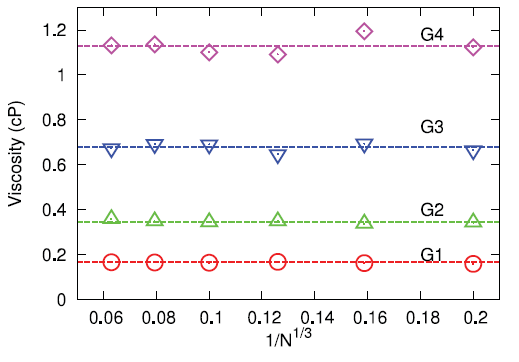
\includegraphics[width=3.2in]{figures/MoultosFig3.png}
	\caption{}
	\label{fig:MoultosFig3}
\end{figure}

\begin{figure}[htb!]
	\centering
	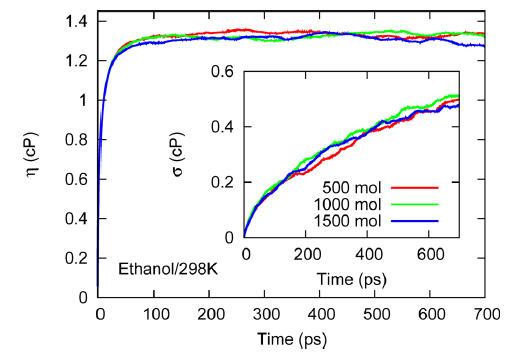
\includegraphics[width=3.2in]{figures/ZhangFig9.png}
	\caption{}
	\label{fig:ZhangFig9}
\end{figure}

\begin{figure}[htb!]
	\centering
	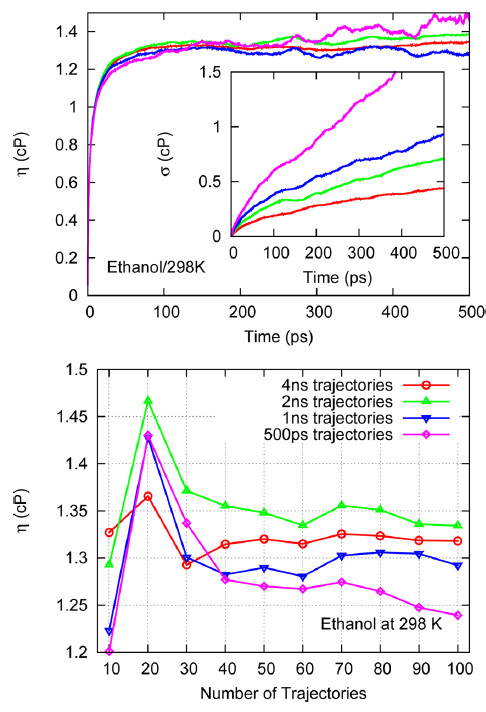
\includegraphics[width=3.2in]{figures/ZhangFig8.png}
	\caption{}
	\label{fig:ZhangFig8}
\end{figure}

\begin{figure}[htb!]
	\centering
	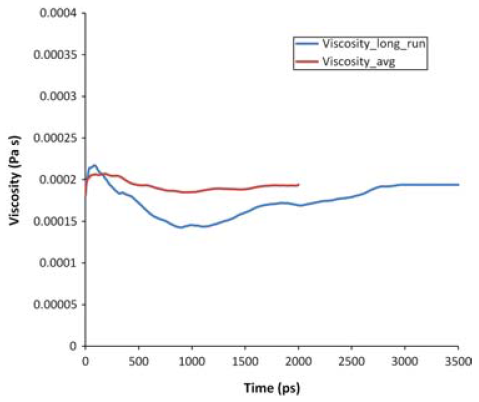
\includegraphics[width=3.2in]{figures/PayalFig2.png}
	\caption{}
	\label{fig:PayalFig2}
\end{figure}

\begin{figure}[htb!]
	\centering
	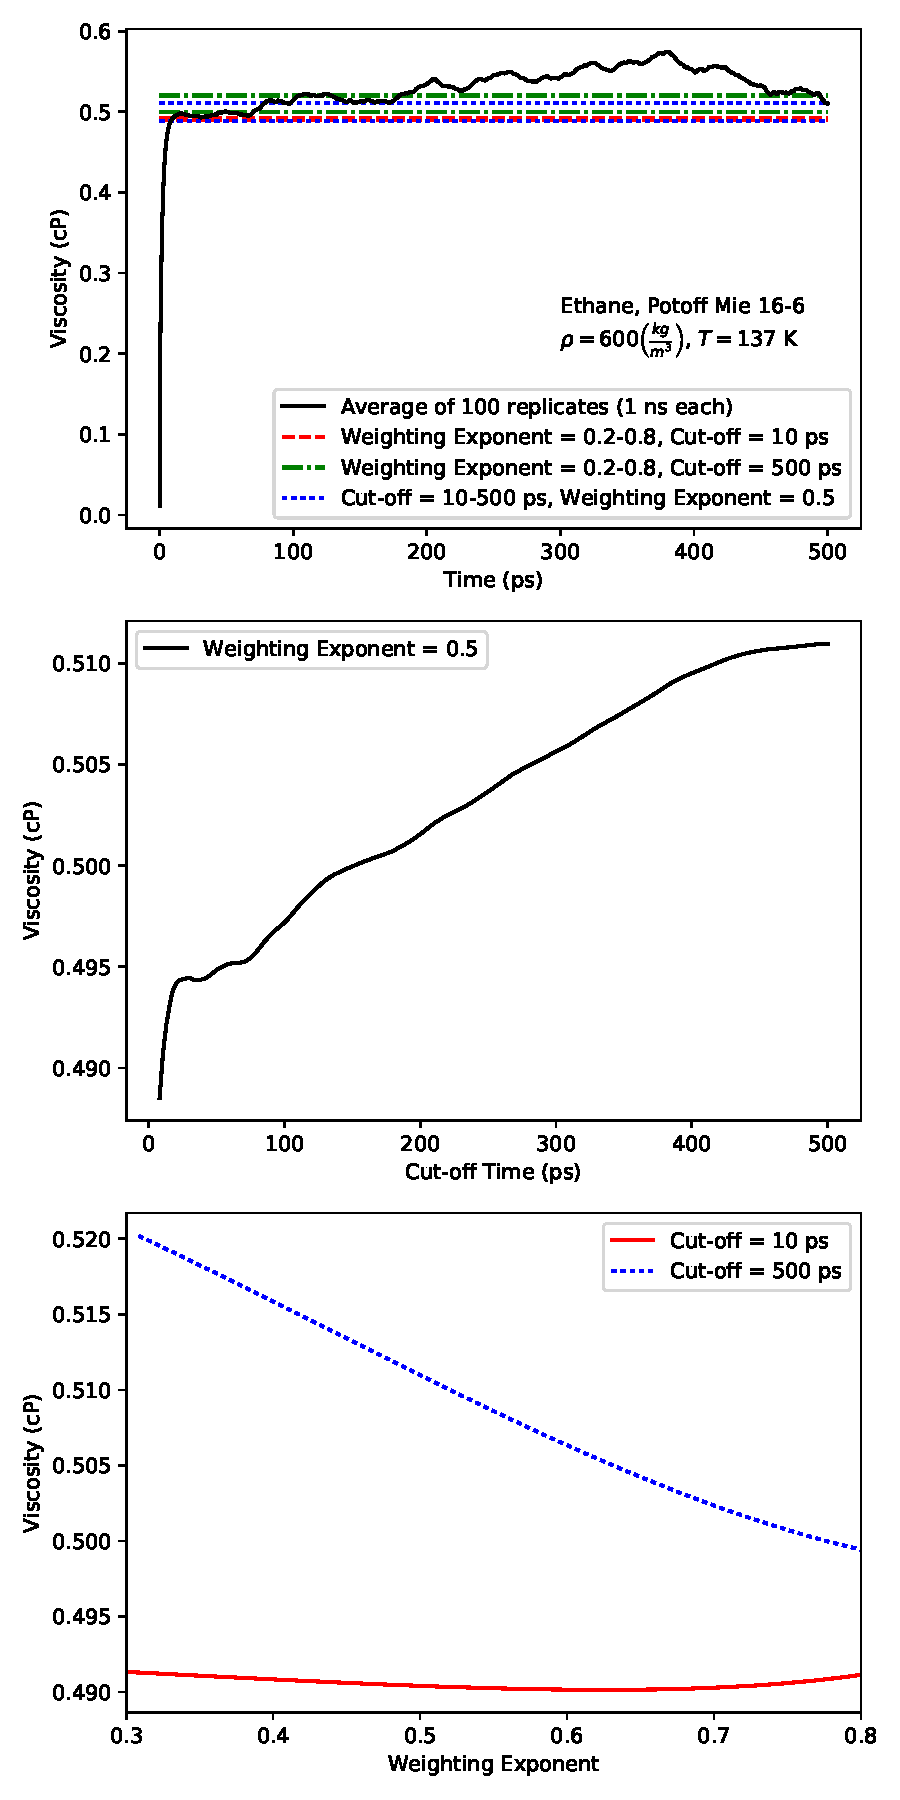
\includegraphics[width=3.2in]{figures/GreenKubo_tcut_b_dependence.pdf}
	\caption{Uncertainty quantification of cut-off time and weighting exponent for method proposed by Zhang et al. Results are shown for a system of 400 united-atom ethane molecules, simulated with the \cite{Potoff2009} model at saturated liquid density for a temperature of 137 K. Top panel plots the Green-Kubo running integral as average of 100 replicates, each of 1 ns duration. The dashed lines represent different estimates of uncertainty attributed to the cut-off time or the weighting exponent. Middle panel plots the estimated viscosity as a function of cut-off time for a fixed weighting exponent. Bottom panel plots the estimated viscosity as a function of the weighting exponent for two different cut-off times. For longer cut-off times, the viscosity depends strongly on the weighting exponent (around $\pm 2$\%) while shorter times are much less dependent (around $\pm 0.1$\%). For the recommended weighting exponent, the cut-off time can cause the viscosity to vary by around $\pm 2$\%. Note that these results may depend strongly on the state point and number of molecules.}
	\label{fig:GK_tcut_b}
\end{figure}

\begin{figure}[htb!]
	\centering
	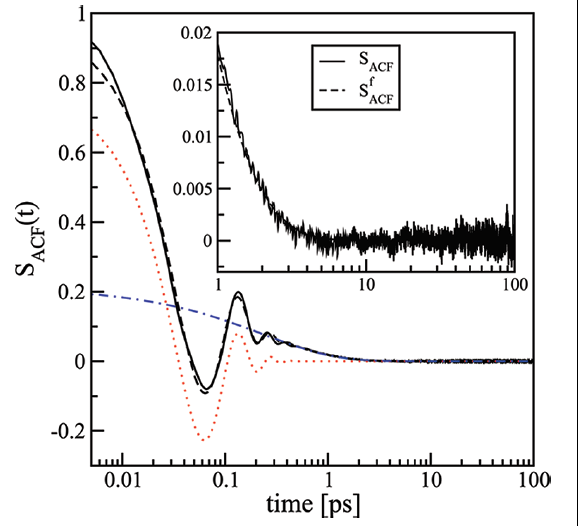
\includegraphics[width=3.2in]{figures/FanourgakisFig1.png}
	\caption{}
	\label{fig:FanourgakisFig1}
\end{figure}

\begin{figure}[htb!]
	\centering
	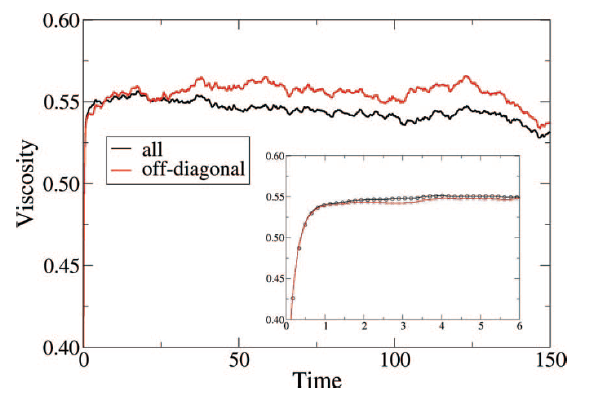
\includegraphics[width=3.2in]{figures/ChenFig1.png}
	\caption{}
	\label{fig:ChenFig1}
\end{figure}

\subsection{Equilibrium Einstein Approach for Viscosity}

Similar to the Einstein approach for self-diffusivity, in general, the initial time should be discarded. Since the Einstein relation is valid in the limit of infinite time, it is common to fit the slope at long time. However, it is also common to fit the slope to an intermediate time interval. We recommend that the author explain why the slope was calculated using a given time interval and how much variability is introduced if a different region is selected.

Similar to the Green-Kubo approach for viscosity, the key to obtaining precise estimates with the Einstein approach is to average multiple replicate simulations. The viscosity with respect to time is estimated from the slope of the Einstein integral. Thus, the average of replicates can be performed in one of two ways. The first option is to calculate the viscosity (i.e. the slope) with respect to time for each replicate and then average the replicate viscosities. However, this approach results in large fluctuations and, therefore, large uncertainties. The second, and recommended, method is to average the Einstein integral of the multiple replicates. The resulting Einstein integral is often linear over a large time interval if sufficient replicates are used. Subsequently, the slope is determined from this average Einstein integral. Fortunately, with sufficient replicate simulations the slope tends to be fairly constant over intermediate and long time intervals. The number of replicates needed has not been rigorously investigated as it has for the Green-Kubo approach. For this reason, we recommend creating a plot of viscosity with respect to number of replicates (see Figure \ref{fig:ZhangFig8}) to determine when sufficient replicates have been simulated. It is our experience that the necessary number of replicates is similar to that for Green-Kubo. As recommended for Green-Kubo, we also recommend bootstrapping the uncertainty. This is done by randomly sampling which replicates are included in the average Einstein integral, calculating the viscosity from the slope, and producing a distribution of these viscosity values from thousands of different random sets of replicates.

Hess claims that the Einstein relation is more convenient than Green-Kubo for viscosity because ``inaccuracies in the long time correlations can be ignored by only considering integral over shorter times.'' 
%What do we want to make of this claim? -RAM

\section{Acknowledgments}

Funder and other information can be given here.

%\nocite{*} % This command displays all refs in the bib file
\bibliography{transport_properties}

%%%%%%%%%%%%%%%%%%%%%%%%%%%%%%%%%%%%%%%%%%%%%%%%%%%%%%%%%%%%
%%% APPENDICES
%%%%%%%%%%%%%%%%%%%%%%%%%%%%%%%%%%%%%%%%%%%%%%%%%%%%%%%%%%%%

\end{document}